\documentclass[10pt,a4papper]{article}
\usepackage{graphicx}
\usepackage{amsmath}
\usepackage{amssymb}
\usepackage{cancel}
\usepackage{multicol}
\usepackage{blindtext}
\usepackage[hidelinks]{hyperref}
\usepackage[left=1.50cm, right=3.00cm, top=2.00cm, bottom=2.00cm]{geometry}
\author{Angel Fdo. García Núñez}
\date{Enero 18, 2023}
\title{Estadisitica}

\begin{document}

\Huge
Calculo de Curvas Geodésicas numéricamente
en superficie Toroide\\

Angel Fernando García Núñez

\Large
\newpage
\[\text{Tensor métrico}\]

\[g_{ij}=(u^k)_i(u^k)_j=\hat e_i\cdot\hat e_j\]\\

\[\text{Símbolos de Chistoffel}\]

\[\text{Primera Clase}\]
\[\Gamma_{jkl}=\frac{1}{2} \left[(g_{jl})_k-(g_{jk})_l+(g_{lk})_j\right]\]

\[\text{Segunda Clase}\]
\[\Gamma_{jk}^i=\frac{1}{2}g^{li}\left[(g_{jl})_k-(g_{jk})_l+(g_{lk})_j\right]=\Gamma_{jkl}g^{li}\]\\

\[\text{Ecuación Geodésica}\]

\[u^i''+\Gamma_{jk}^iu^j'u^k'=0\]

\newpage
\[\text{Parametrización de un toro}\]

\[\vec x(u^1,u^2)=\left[(R+r\cos u^1)\cos u^2,(R+r\cos u^1)\sin u^2,r\sin u^1\right]\]\\

\[\text{Vectores tangentes}\]

\[\hat e_1=\frac{\partial\vec x}{\partial u^1}=\left[-r\sin u^1\cos u^2,-r\sin u^1\sin u^2,r\cos u^1\right]\]

\[\hat e_2=\frac{\partial\vec x}{\partial u^2}=\left[-(R+r\cos u^1)\sin u^2,(R+r\cos u^1)\cos u^2,0\right]\]

\[\text{Tensor métrico}\]

\[g_{11}=\hat e_1\cdot\hat e_1=r^2\sin^2 u^1\cos^2 u^2+r^2\sin^2 u^1\sin^2 u^2+r^2\cos^2 u^1=r^2\]

\[g_{12}=\hat e_1\cdot\hat e_2=(R+r\cos u^1)r\sin u^1\cos u^2\sin u^2-(R+r\cos u^1)r\sin u^1\sin u^2\cos u^2=0\]

\[g_{21}=\hat e_2\cdot\hat e_1=\hat e_1\cdot\hat e_2=g_{12}=0\]

\[g_{22}=\hat e_2\cdot\hat e_2=(R+r\cos u^1)^2\sin^2 u^2+(R+r\cos u^1)^2\cos^2 u^2=(R+r\cos u^1)^2\]

\[g_{ij}=\begin{bmatrix}
r^2 & 0\\
0 & (R+r\cos u^1)^2
\end{bmatrix}\]

\[\text{Derivadas parciales del tensor métrico}\]

\[(g_{ij})_1=\begin{bmatrix}
0 & 0\\
0 & -2r(R+r\cos u^1)\sin u^1
\end{bmatrix}\quad,\quad
(g_{ij})_2=\begin{bmatrix}
0 & 0\\
0 & 0
\end{bmatrix}\]

\newpage
\[\text{Tensor métrico contra variante}\]

\[g^{ij}=\frac{1}{g}\text{cof}(g_{ij})\]

\[g=|g_{ij}|=r^2(R+r\cos u^1)^2\quad,\quad
\text{cof}(g_{ij})=
\begin{bmatrix}
(R+r\cos u^1)^2 & 0\\
0 & r^2
\end{bmatrix}\]

\[g^{ij}=
\begin{bmatrix}
\frac{1}{r^2} & 0\\
0 & \frac{1}{(R+r\cos u^1)^2}
\end{bmatrix}\]\\

\[\text{Símbolos de Chistoffel}\]

\[\Gamma_{11}^1=\frac{1}{2}g^{11}\left[(g_{11})_1-(g_{11})_1+(g_{11})_1\right]+\frac{1}{2}g^{21}\left[(g_{12})_1-(g_{11})_2+(g_{21})_1\right]\]

\[\Gamma_{11}^1=\frac{1}{2r^2}(0-0+0)+0(0-0+0)=0\]\\

\[\Gamma_{12}^1=\Gamma_{21}^1=\frac{1}{2}g^{11}\left[(g_{11})_2-(g_{12})_1+(g_{12})_1\right]+\frac{1}{2}g^{21}\left[(g_{12})_2-(g_{12})_2+(g_{22})_1\right]\]

\[\Gamma_{12}^1=\Gamma_{21}^1=\frac{1}{2r^2}(0-0+0)+0(0-0-2r(R+r\cos u^1)\sin u^1)=0\]\\

\[\Gamma_{11}^2=\frac{1}{2}g^{12}\left[(g_{11})_1-(g_{11})_1+(g_{11})_1\right]+\frac{1}{2}g^{22}\left[(g_{12})_1-(g_{11})_2+(g_{21})_1\right]\]

\[\Gamma_{11}^2=0(0-0+0)+\frac{1}{2(R+r\cos u^1)^2}(0-0+0)=0\]

\newpage
\[\Gamma_{12}^2=\Gamma_{21}^2=\frac{1}{2}g^{12}\left[(g_{11})_2-(g_{12})_1+(g_{12})_1\right]+\frac{1}{2}g^{22}\left[(g_{12})_2-(g_{12})_2+(g_{22})_1\right]\]

\[\Gamma_{12}^2=\Gamma_{21}^2=0(0-0+0)+\frac{1}{2(R+r\cos u^1)^2}(0-0-2r(R+r\cos u^1)\sin u^1)=-\frac{r\sin u^1}{(R+r\cos u^1)}\]\\

\[\Gamma_{22}^1=\frac{1}{2}g^{11}\left[(g_{21})_2-(g_{22})_1+(g_{12})_2\right]+\frac{1}{2}g^{21}\left[(g_{22})_2-(g_{22})_2+(g_{22})_2\right]\]

\[\Gamma_{22}^1=\frac{1}{2r^2}(0+2r(R+r\cos u^1)\sin u^1+0)+0(0+0)=\frac{(R+r\cos u^1)\sin u^1}{r}\]\\

\[\Gamma_{22}^2=\frac{1}{2}g^{12}\left[(g_{21})_2-(g_{22})_1+(g_{12})_2\right]+\frac{1}{2}g^{22}\left[(g_{22})_2-(g_{22})_2+(g_{22})_2\right]\]

\[\Gamma_{22}^2=0(0+2r(R+r\cos u^1)\sin u^1+0)+\frac{1}{2(R+r\cos u^1)^2}(0-0+0)=0\]\\

\newpage
\[\text{Ecuaciones Geodésicas}\]

\[u^1''+\Gamma_{22}^1u^2'u^2'=0\quad\to\quad
u^1''+\frac{(R+r\cos u^1)\sin u^1}{r}u^2'u^2'=0\]

\[u^2''+\Gamma_{12}^2u^1'u^2'=0\quad\to\quad
u^2''-\frac{r\sin u^1}{(R+r\cos u^1)}u^1'u^2'=0\]

\newpage
Solución numérica

\[\text{Sistema de ecuaciones diferenciales de primer orden}\]

\[y_1'=u_1'=y_2\]

\[y_2'=u_1''=-\frac{(R+r\cos y^1)\sin y^1}{r}y_4^2\]

\[y_3'=u_2'=y_4\]

\[y_4'=u_2''=\frac{r\sin y^1}{(R+r\cos y^1)}y_2y_4\]\\

\[\vec y=
\begin{pmatrix}
  y_1\\
  y_2\\
  y_3\\
  y_4
\end{pmatrix}\quad,\quad
\vec f(\vec y)=
\begin{pmatrix}
  y_2\\
  -\frac{(R+r\cos y^1)\sin y^1}{r}y_4^2\\
  y_4\\
  \frac{r\sin y^1}{(R+r\cos y^1)}y_2y_4
\end{pmatrix}\quad:\quad
\vec f(\vec y)=\vec{y'}\]\\

\[\text{Método Runge-Kutta de cuarto orden}\]

\[\vec k_1=\vec f(\vec y_i)\]

\[\vec k_2=\vec f\left(\vec y_i+\frac{h}{2}\vec k_1\right)\]

\[\vec k_3=\vec f\left(\vec y_i+\frac{h}{2}\vec k_2\right)\]

\[\vec k_4=\vec f\left(\vec y_i+h\vec k_3\right)\]

\[\vec y_{i+1}=\vec y_i+\frac{h}{6}\left(\vec k_1+2\vec k_2+2\vec k_3+\vec k_4\right)\]

\newpage
\[\text{Solución numérica programada en Python, para los puntos:}\]
\[P_1=\vec x\left(\frac{\pi}{2},0\right)=(4,0,2)\quad,\quad
P_2=\vec x\left(\frac{3}{2}\pi,\pi\right)=(-4,0,-2)\]

\[\text{Velocidades iniciales obtenidas:}\quad
\alpha=0.4968\quad,\quad
\beta=0.1926\]
\[\text{Error mínimo obtenido:}\quad
\Delta=0.0058\]

\[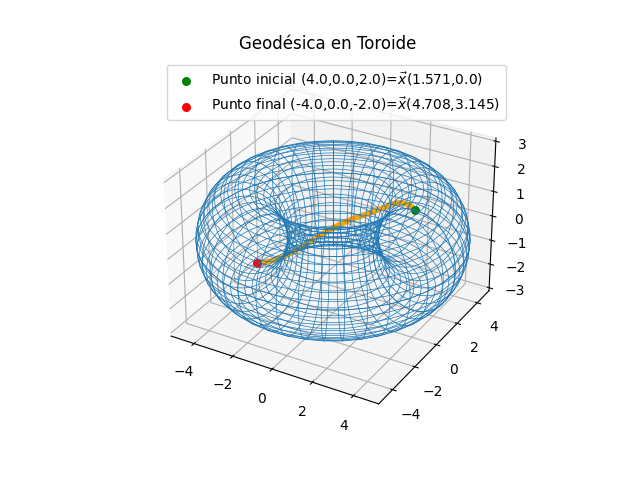
\includegraphics[scale=0.7]{p1-1.png}\]
\[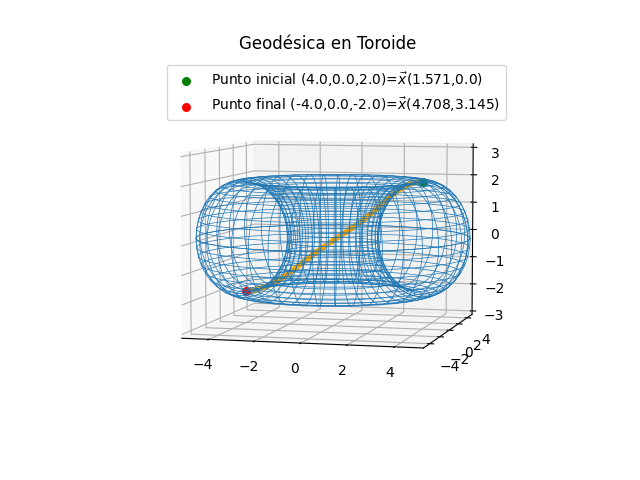
\includegraphics[scale=0.7]{p1-2.png}\]

\newpage
\[\text{Solución numérica programada en Python, para los puntos:}\]
\[P_1=\vec x\left(\frac{\pi}{2},0\right)=(4,0,2)\quad,\quad
P_2=\vec x\left(\pi,\pi\right)=(-2,0,0)\]

\[\text{Velocidades iniciales obtenidas:}\quad
\alpha=0.4263\quad,\quad
\beta=0.18\]
\[\text{Error mínimo obtenido:}\quad
\Delta=0.038\]

\[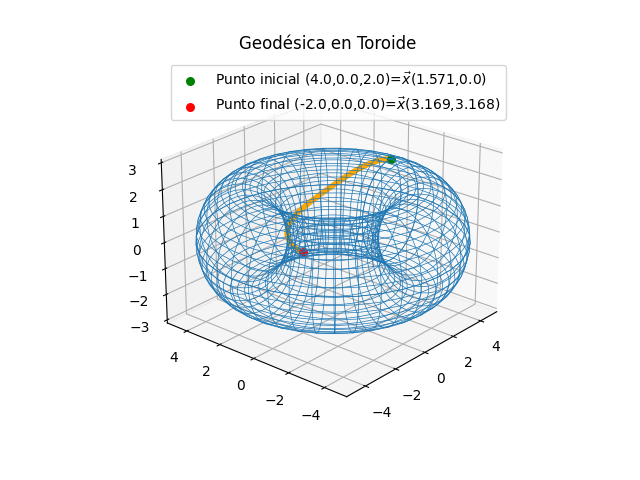
\includegraphics[scale=0.7]{p2-3.png}\]
\[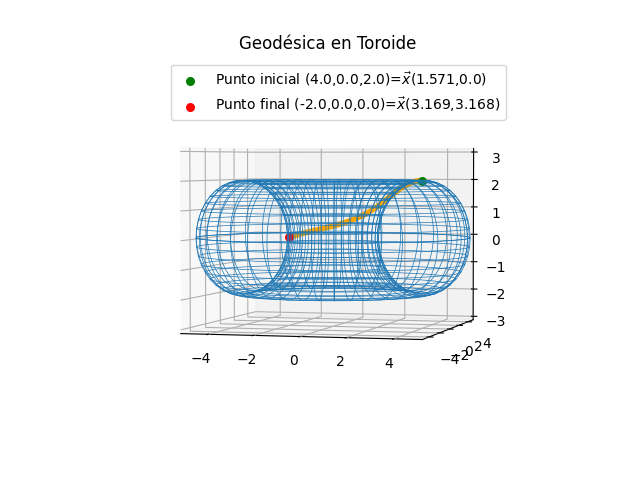
\includegraphics[scale=0.7]{p2-2.png}\]

\newpage
\[\text{Solución numérica programada en Python, para los puntos:}\]
\[P_1=\vec x\left(\frac{\pi}{2},0\right)=(4,0,2)\quad,\quad
P_2=\vec x\left(\frac{\pi}{2},\pi\right)=(-4,0,2)\]

\[\text{Velocidades iniciales obtenidas:}\quad
\alpha=0.4526\quad,\quad
\beta=0.0.2105\]
\[\text{Error mínimo obtenido:}\quad
\Delta=0.0323\]

\[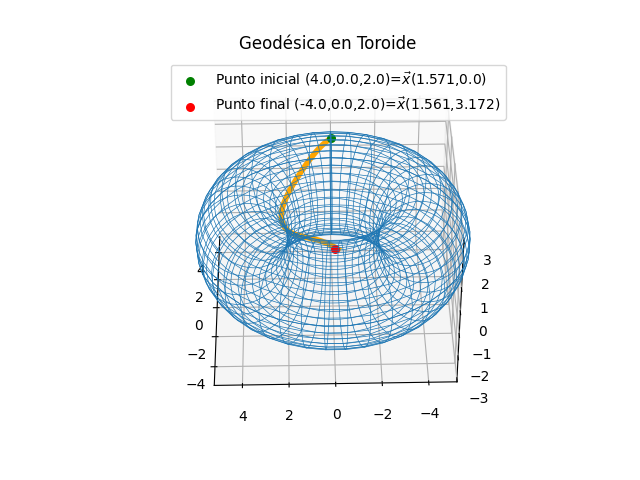
\includegraphics[scale=0.7]{p3-5.png}\]
\[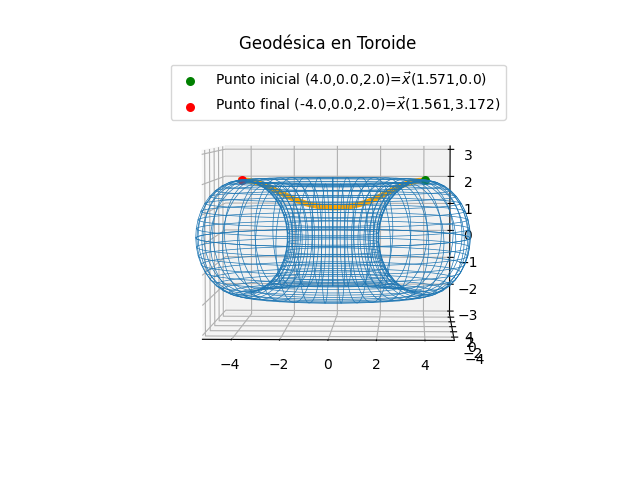
\includegraphics[scale=0.7]{p3-4.png}\]

\newpage
\[\text{Solución numérica programada en Python, para los puntos:}\]
\[P_1=\vec x\left(\frac{\pi}{2},\pi\right)=(4,0,2)\quad,\quad
P_2=\vec x\left(\frac{3}{2}\pi,\pi\right)=(-4,0,-2)\]

\[\text{Velocidades iniciales obtenidas:}\quad
\alpha=0.3158\quad,\quad
\beta=0\]
\[\text{Error mínimo obtenido:}\quad
\Delta=0.0131\]

\[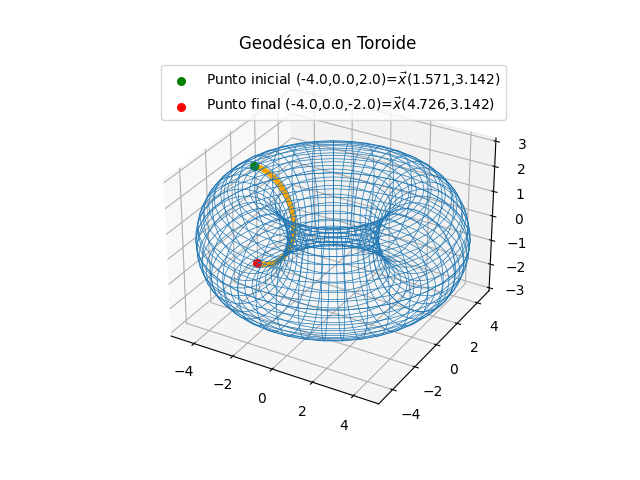
\includegraphics[scale=0.7]{p4-1.png}\]
\[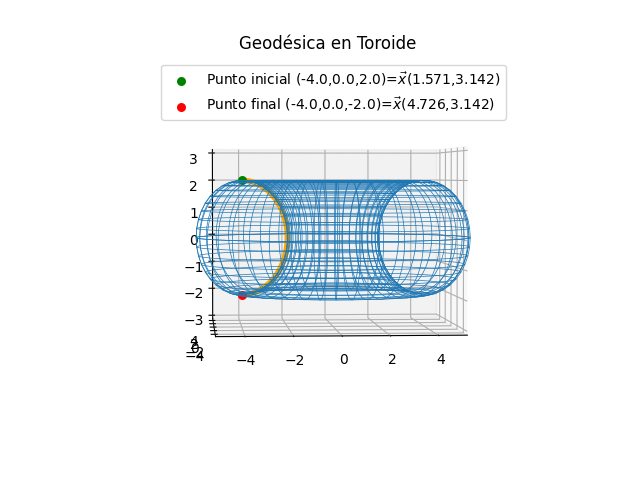
\includegraphics[scale=0.7]{p4-2.png}\]

\newpage
\[\text{Solución numérica programada en Python, para los puntos:}\]
\[P_1=\vec x\left(0,0\right)=(6,0,0)\quad,\quad
P_2=\vec x\left(0,\pi\right)=(-6,0,0)\]

\[\text{Velocidades iniciales obtenidas:}\quad
\alpha=0\quad,\quad
\beta=0.3158\]
\[\text{Error mínimo obtenido:}\quad
\Delta=0.0131\]

\[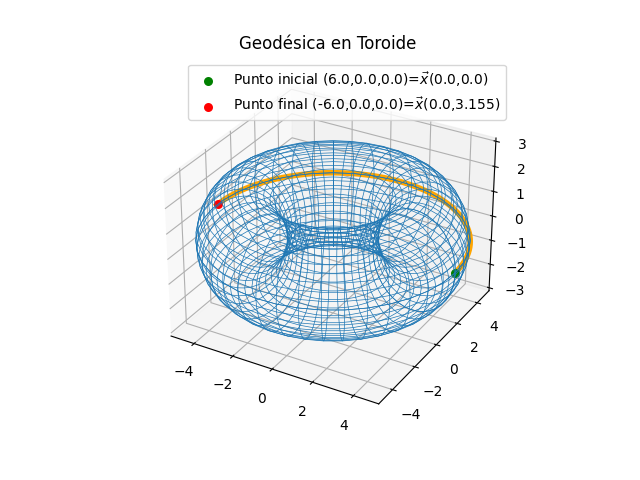
\includegraphics[scale=0.7]{p5-1.png}\]
\[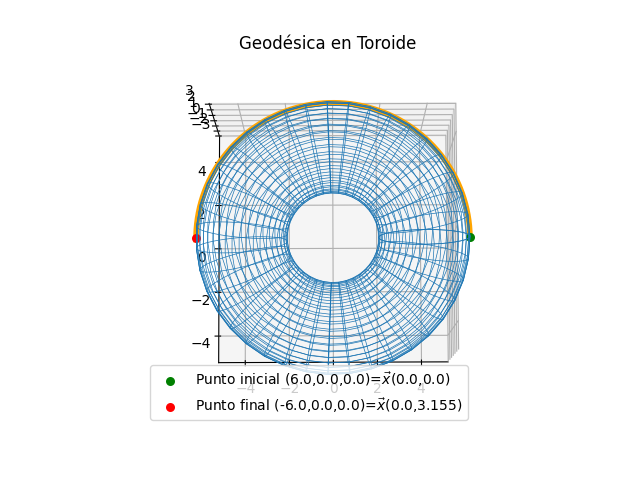
\includegraphics[scale=0.7]{p5-2.png}\]

\newpage
\[\text{Solución numérica programada en Python, para los puntos:}\]
\[P_1=\vec x\left(0,0\right)=(6,0,0)\quad,\quad
P_2=\vec x\left(\pi,\pi\right)=(-2,0,0)\]

\[\text{Velocidades iniciales obtenidas:}\quad
\alpha=0.6368\quad,\quad
\beta=0.1421\]
\[\text{Error mínimo obtenido:}\quad
\Delta=0.0251\]

\[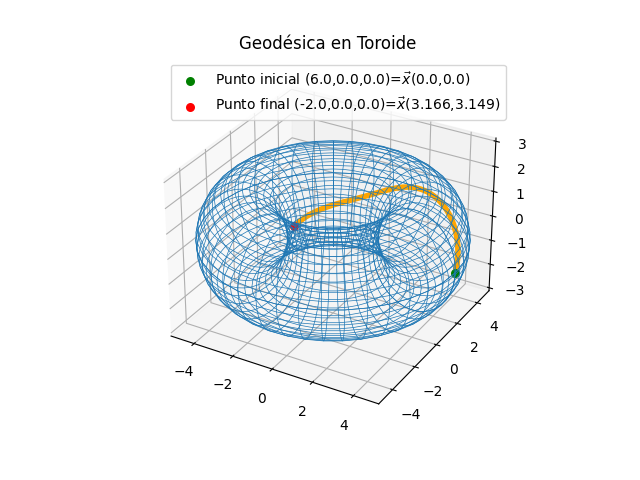
\includegraphics[scale=0.7]{p6-1.png}\]
\[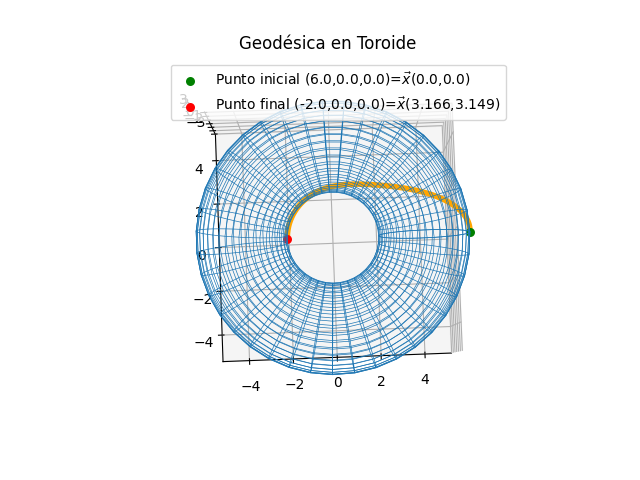
\includegraphics[scale=0.7]{p6-2.png}\]

\newpage
\[\text{Solución numérica programada en Python, para los puntos:}\]
\[P_1=\vec x\left(0,0\right)=(6,0,0)\quad,\quad
P_2=\vec x\left(\frac{3.5}{2}\pi,\pi\right)=(-5.414,0,-1.414)\]

\[\text{Velocidades iniciales obtenidas:}\quad
\alpha=0.7753\quad,\quad
\beta=0.1558\]
\[\text{Error mínimo obtenido:}\quad
\Delta=0.0077\]

\[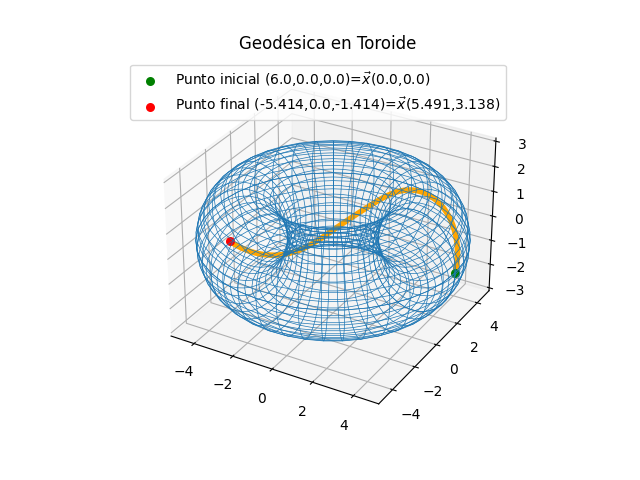
\includegraphics[scale=0.7]{p7-1.png}\]
\[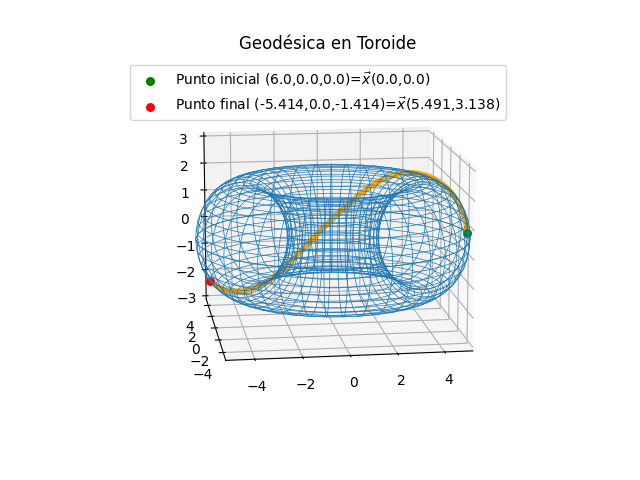
\includegraphics[scale=0.7]{p7-2.png}\]

\newpage

\newpage

\newpage

\newpage

\newpage

\newpage

\newpage

\newpage

\newpage

\newpage

\newpage

\newpage

\newpage

\newpage

\newpage

\newpage

\newpage

\newpage

\newpage

\newpage

\newpage

\newpage

\newpage

\newpage

\newpage

\newpage

\newpage

\newpage

\newpage

\newpage

\newpage

\newpage

\newpage

\newpage

\newpage

\newpage

\newpage

\newpage

\newpage

\newpage

\newpage

\newpage

\newpage

\newpage

\newpage

\newpage

\newpage

\newpage

\newpage

\newpage

\newpage

\newpage

\newpage

\newpage

\newpage

\newpage

\newpage

\newpage

\newpage

\newpage

\newpage

\newpage

\newpage

\newpage

\newpage

\newpage

\newpage

\newpage

\newpage

\newpage

\newpage

\newpage

\newpage

\newpage

\newpage

\newpage

\newpage

\newpage

\newpage

\newpage

\newpage

\newpage

\newpage

\newpage

\newpage

\newpage

\newpage

\newpage

\newpage

\newpage

\newpage

\newpage

\newpage

\newpage

\newpage

\newpage

\newpage

\newpage

\newpage

\newpage

\newpage

\newpage

\newpage

\newpage

\newpage

\newpage

\newpage

\newpage

\newpage

\newpage

\newpage

\newpage


\end{document}
